\section{Ejercicio 3}
\subsection*{Instrucción}
Cuando los clientes de la empresa de alquiler de coches alquilan un coche, el sistema que estamos construyendo
tiene que proporcionarles el precio del alquiler. Este precio lo calcula la operación \texttt{getPrice() : Integer} de la siguiente
forma: El precio base será el precio del modelo del vehículo por día.
\begin{center}
    \texttt{ (pricePerDay) * [endDate - startDate]}
\end{center}
Además, la empresa de alquiler de coches puede añadir al cálculo de precios la posibilidad de hacer promociones
que implican descuentos de estos precios. Inicialmente, la empresa ofrecerá dos tipos de promociones: por cantidad
y por porcentaje.
\begin{itemize}
    \item \textbf{Promoción por cantidad:} permitirá decrementar el precio del alquiler en la cantidad indicada en
    la promoción.
    \item \textbf{Promoción por porcentaje:} decrementará el precio del alquiler en el porcentaje indicado en la
    promoción. Las promociones se asignan a los alquileres en el momento de su creación.
\end{itemize}
Evidentemente, es posible
que a algunos alquileres no se les aplique ninguna promoción. Las promociones que se asignan a los alquileres son
determinadas por una política de la empresa que no impacta al diseño de nuestra operación (impactará a la
operación que crea los alquileres).\par
\vspace{0.15cm}
Eso sí, la empresa quiere que mientras no se haga el pago del alquiler, si aparecen
nuevas promociones, se apliquen a los alquileres siempre y cuando sean más favorables (no nos tenemos que
preocupar tampoco de estos cambios, son gestionados por otras operaciones).


\subsection{Patrón de Diseño utilizado}
En un principio teniamos pensado usar el patrón visitante pero al final la acabamos descartando porque nos estaba siendo muy complicado 
pensar la solución con este patrón y además era muy complejo de implementar.\par
Al final cabamos optando por usar el patrón estrategia ya que es un patrón relativamente simple que nos permitia añadir el algoritmo para calcular 
los descuentos de una manera sencilla y rápida de llevar a cabo, en nuestro problema hemos implementado una interfaz con la operación de 
aplicar descuento y dos clases distintas una para descuentos de promociones y otra de porcentajes que veremos con más detalle en el diagrama. \par

\subsection{Efectos sobre el Diagrama de Diseño}

\begin{figure}[H]
    \centering
     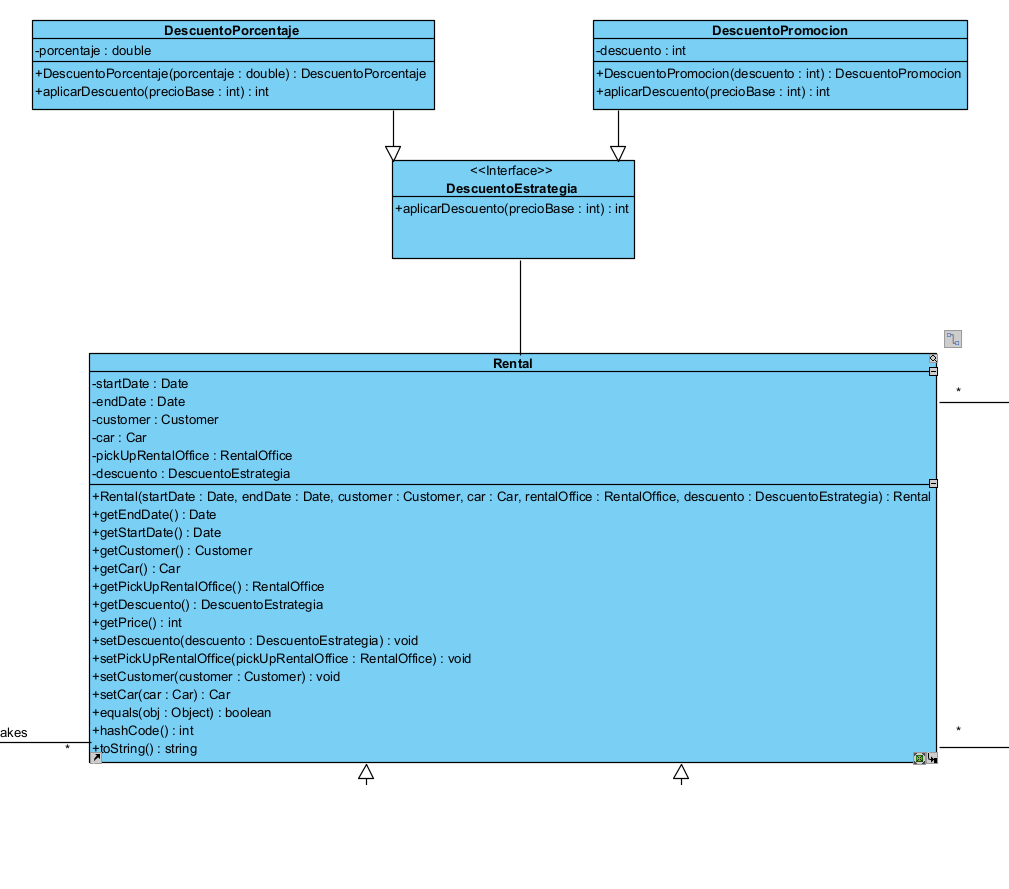
\includegraphics[width=1\linewidth]{assets/diagramas/UML_Apartado3.png}
     \caption{Diagrama de Diseño centrado en lo nuevo del apartado 3}
\end{figure}

Como podemos observar 

\subsection{Implementación de \textit{getPrice() : Integer}}
\begin{lstlisting}[style = javaNormal, language=Java] 

    introducir codigo aqui

\end{lstlisting} % Código en el documento "codigosEj3"

\newpage
